\documentclass[
	handout,
%  	aspectratio=43
  	aspectratio=169
]{beamer}

\usepackage[utf8]{inputenc}
\usepackage[german]{babel}
\usepackage[figurename=Bild]{caption}
\usepackage{graphicx}
\usepackage{amsmath}
\usepackage{scrextend}
\usepackage{xcolor,colortbl}	
\usepackage{lmodern}	
\usepackage{amsmath,amssymb}
\usepackage{booktabs}

\title[Semesterprojekt KNIME]{Data Mining}

\date{18.06.2021}
\author[C. Werner, J. Prothmann]{C. Werner, J. Prothmann}


\institute{Bereich Elektrotechnik und Informatik}
\usetheme{Wismar}	% Design der Hochschule Wismar
\usecolortheme{FIW}

% Die Navigationshilfen unteren Folienrand kann man ausblenden
\beamertemplatenavigationsymbolsempty
% \beamertemplatefootempty

% Wenn mathematische Umgebungen in klassischer "Mathe-Schrift"
% dargestellt werden sollen, folgende Zeile entkommentieren.
%\usefonttheme[onlymath]{serif}

% Zeige Abschnittstitel auf separater Folie vor jedem Abschnitt
%\AtBeginSection{\frame{\sectionpage}}

\begin{document}
	\begin{frame}[plain]
		\titlepage
	\end{frame}

	\begin{frame}[allowframebreaks]{Gliederung}
		\tableofcontents
	\end{frame}

	\section{Vorverarbeitung}
	\frame{\sectionpage}
		
		\begin{frame}{Rohdatensatz}
			\begin{figure}[!h]
				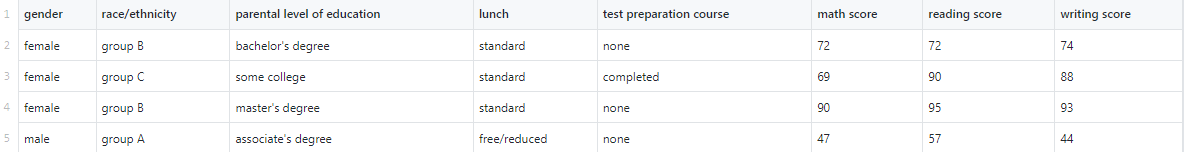
\includegraphics[scale= 0.55]{../pictures/roh.png}
				\caption{Rohdatensatz}
			\end{figure}
		\end{frame}

		\begin{frame}{Datenvorverarbeitung}
			\begin{figure}[!h]
				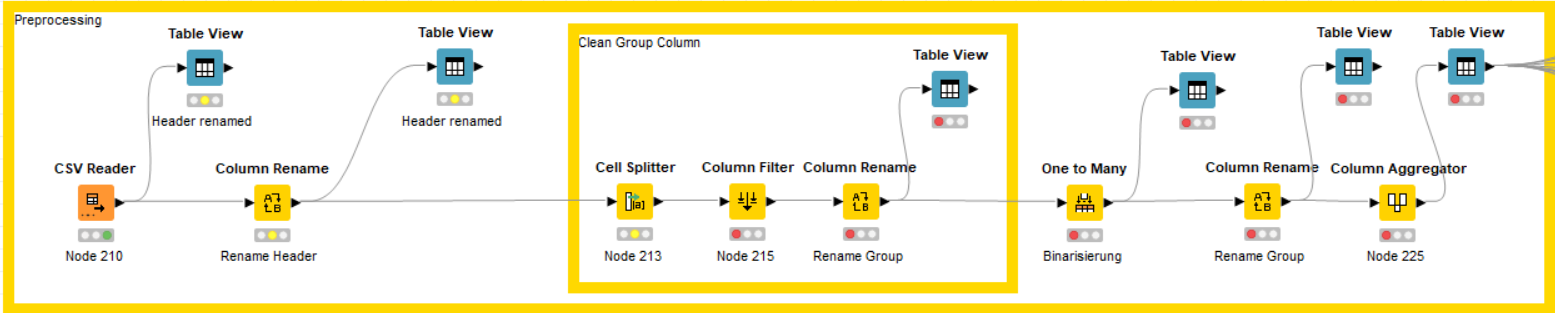
\includegraphics[scale= 0.4]{../pictures/preprocessing.png}
				\caption{Knime Workflow zur Vorverarbeitung}
			\end{figure}
		\end{frame}

		\begin{frame}
			\begin{figure}[!h]
				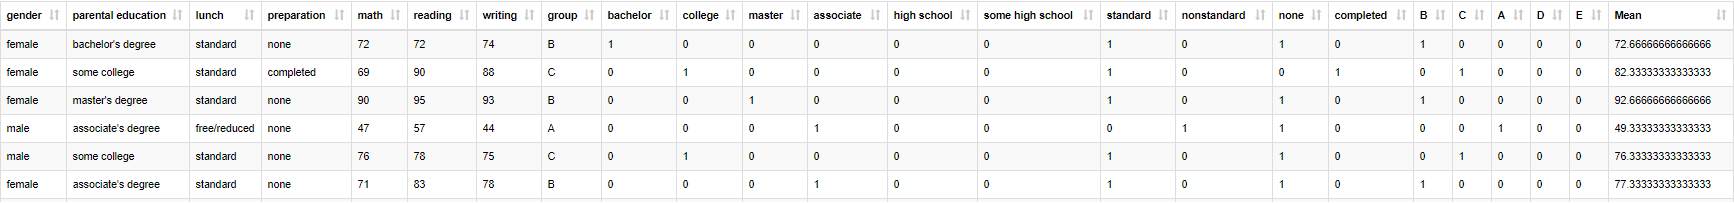
\includegraphics[scale= 0.4]{../pictures/processed.png}
				\caption{Vorverarbeitete Daten}
			\end{figure}
		\end{frame}

	\section{Entscheidungsbäume}	
	\frame{\sectionpage}
	
		\begin{frame}{Decision Tree Learner}
			\begin{itemize}
				\item Standardknoten von Knime
				\item Zielattribut: nominal
				\item Entscheidungsfindungsattribute: nominal, numerisch
				\item Qualitätsmaße für Splitberechnung:
				\begin{itemize}
					\item Gini-Index
					\item Gain-Ratio
				\end{itemize}
				\item Pruning möglich
			\end{itemize}
		\end{frame}

		\begin{frame}{SimpleCart}	
			\begin{itemize}
				\item Weka-Knoten
				\item Erzeugung von Binärbäumen
				\item Pruning möglich
				\item Je höher der Informationsgehalt eines Attributs in Bezug auf die Zielgröße, desto weiter oben im Baum findet
sich dieses Attribut. 
			\end{itemize}
			\begin{center}
				\begin{figure}[h]
					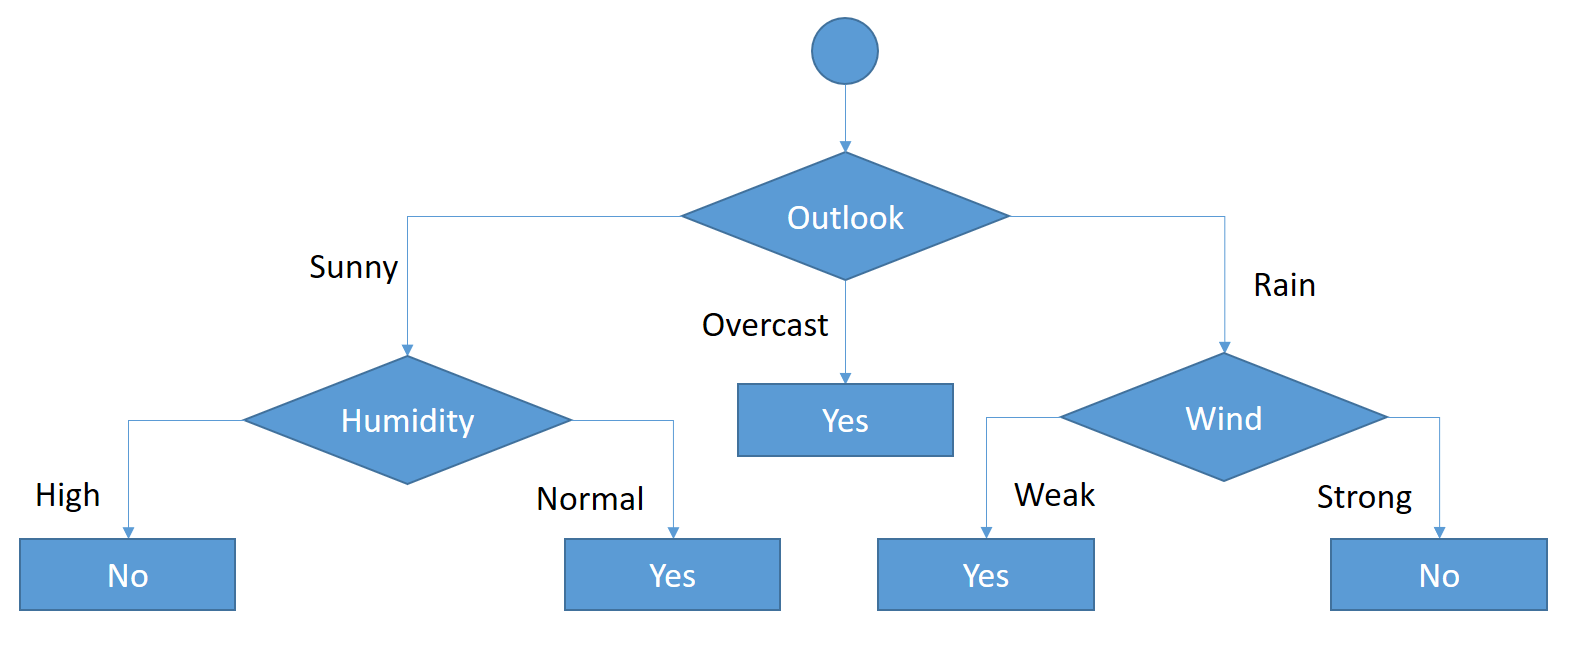
\includegraphics[scale=0.2]{../pictures/cart-tree.png}
					\caption{CART Tree Beispiel}		
				\end{figure}		
			\end{center}
		\end{frame}

		\begin{frame}{J48}		
			\begin{itemize}
				\item Weka-Knoten
				\item C4.5 Algorithmus von J. Ross Quinlan
				\item Ähnlich zu CART, jedoch kein Binärbaum
				\item Deutlich breiter und weniger tief als CART
				\item Pruning möglich
			\end{itemize}
		\end{frame}

		\begin{frame}{NBTree}
			\begin{itemize}
				\item Weka-Knoten
				\item Hybridalgorithmus aus Entscheidungsbaum- und Naive-Bayes-Klassifikatoren
				\item \glqq{}klassische\grqq{} Knoten
				\item Blätter enthalten Naive-Bayes’sche Klassifikatoren
			\end{itemize}	
			
			\begin{center}
				\begin{figure}[h]
					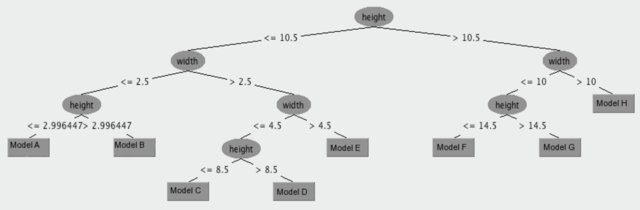
\includegraphics[scale=1]{../pictures/NBTree-classifying-MAC-Felinae.jpg}
					\caption{NB Tree Beispiel}		
				\end{figure}		
			\end{center}			
		\end{frame}

		\begin{frame}{REPTree}	
			\begin{itemize}
				\item Weka-Knoten
				\item basiert auf C4.5 Algorithmus
				\item Generierung unter Berücksichtigung von:
				\begin{itemize}
					\item Informationsgewinn
					\item Varianz
				\end{itemize}
			\end{itemize}	
		\end{frame}

		\begin{frame}{LMT}	
			\begin{itemize}
				\item Weka-Knoten
				\item Blätter: lineare Regressionsfunktionen
				\item stufenweiser Anpassungsprozess
				\item Automatische Auswahl relevanter Attribute
			\end{itemize}		
		\end{frame}

		\begin{frame}{DecisionStump}		
			\begin{itemize}
				\item Weka-Knoten
				\item einstufiger Entscheidungsbaum
				\item Vorhersage anhand des Wertes eines Eingabe-Features
				\item Knoten: Schwellenwert
				\item Blätter: Werte unterhalb und oberhalb des Schwellenwerts
				\item Einsatz als \glqq{}schwache Lerner\grqq{} (z.B. Gesichtserkennung)
			\end{itemize}
		\end{frame}

		\begin{frame}{J48Graft}	
			\begin{itemize}
				\item Weka-Knoten
				\item nutzt den C4.5++ Algortihmus
				\item Verbesserung durch \glqq{}all-tests-but-one-partition\grqq{} (ATBOP)
				\item Reduzierte Rechenzeit
				\item Reduzierte Komplexität des Baums
			\end{itemize}	
		\end{frame}

		\begin{frame}{BFTree}	
			\begin{itemize}
				\item Weka-Knoten
				\item Best-First-Entscheidungsbaum
				\item \glqq{}beste\grqq{} Knoten zuerst expandieren
				\item \glqq{}beste\grqq{} Knoten: maximalen Reduktion der Unreinheit (z.B. Gini-Index)
				\item resultierende Baum nur in Reihenfolge unterschiedlich
			\end{itemize}		
		\end{frame}

		\begin{frame}{RandomTree}	
			\begin{itemize}
				\item Weka-Knoten
				\item zufällig ausgewählte Attribute an den Knoten
				\item kein Pruning
			\end{itemize}		
		\end{frame}

		\begin{frame}{RandomForest}		
			\begin{itemize}
				\item Weka-Knoten
				\item Kombination von Baumprädiktoren
				\item Abhängigkeit jedes Baumes von Werten eines Zufallsvektors
				\item Zufallsvektor: unabhängig und besitzt gleiche Verteilung für alle Bäume im ‘Wald’
			\end{itemize}	
		\end{frame}
	
	\section{Cluster}	
	\frame{\sectionpage}	
		
		\begin{frame}{Cluster}
			\begin{itemize}
				\item kMeans
				\item Dichtebasiertes Clustern
				\item Hierarchisches Clustern
			\end{itemize}
		\end{frame}
		
		\begin{frame}{kMeans Algortihmus}
			\begin{itemize}
				\item 3 Schritte: 1. Initialisierung, 2. Zuordnung, 3. Aktualisierung
				\item Wiederholen von Schritt 2 und 3 bis Abbruchbedingun erreicht
				\item kMeans Knoten ist in Auslieferungsversion von KNIME enthalten
				\item Keine dynamische Anzahl an Cluster
				\item Abbruchbedingung entweder max Iterationen oder Schritt 2 und 3 bringen keine Änderungen mehr
				\item Distanzberechnung mit euklidischer Distanz (Lineare Distanz von 2 Punkten im Raum)
			\end{itemize}
		\end{frame}
		
		\begin{frame}{Dichtebasiertes Clustern}
			\begin{itemize}
				\item DBSCAN Knoten in KNIME
				\item Density-Based Spatial Clustering of Applications with Noise
				\item Unterteilung der Daten in 3 Kategorien: Core Punkte, Border Punkte, Noise Punkte
				\item Clusterbildung durch verbinden von Core Punkten
				\item Punkte innerhalb der Core Punkte - Distanz zählen zum Cluster, alle außerhalb sind Noise
			\end{itemize}
		\end{frame}
		
		\begin{frame}{~}
			\begin{center}
				\begin{figure}[h]
					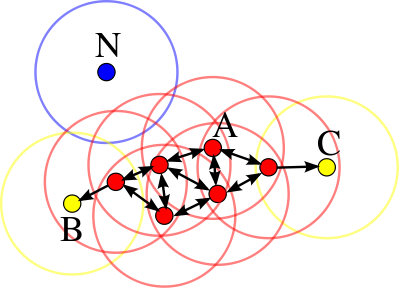
\includegraphics[scale=0.5]{../pictures/dbscan.png}
					\caption{DBSCAN Algorithmus}		
				\end{figure}		
			\end{center}	
		\end{frame}
		
		\begin{frame}{Hierarchisches Clustern}
			\begin{itemize}
				\item Sowohl Build-In Knoten als auch WEKA Extension
				\item Berechnen der Punktdistanzen durch diverse Distanzmaße (Euklidische-, Manhatten-, ...-Distanz)
				\item Beide Knoten sind agglomerativ (bottom-up): Iterative Bildung von großen Clustern aus bestehenden
				\item Darstellung in Dendrogrammen
			\end{itemize}
		\end{frame}
		
		\begin{frame}{Silhouettenkoeffizient}
			\begin{itemize}
				\item Berechnet die Qualität von Clustern
				\item Berechnent für jede Zeile wie gut das ausgewählte Cluster passt
				\item Reichweite von -1 bis 1 $\rightarrow$ je höher der Wert, desto besser die Clusterung
			\end{itemize}
			\begin{center}
				\begin{figure}[h]
					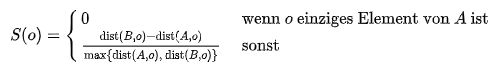
\includegraphics[scale=1]{../pictures/formel.png}
					\caption{Formel Silhouettenkoeffizient}		
				\end{figure}		
			\end{center}	
		\end{frame}
	
	\section{Implementierung}	
	\frame{\sectionpage}
	
		\subsection{Entscheidungsbäume}
			\begin{frame}{Gesamtworkflow Entscheidungsbäume}
				\begin{center}					
					\begin{figure}[h]
						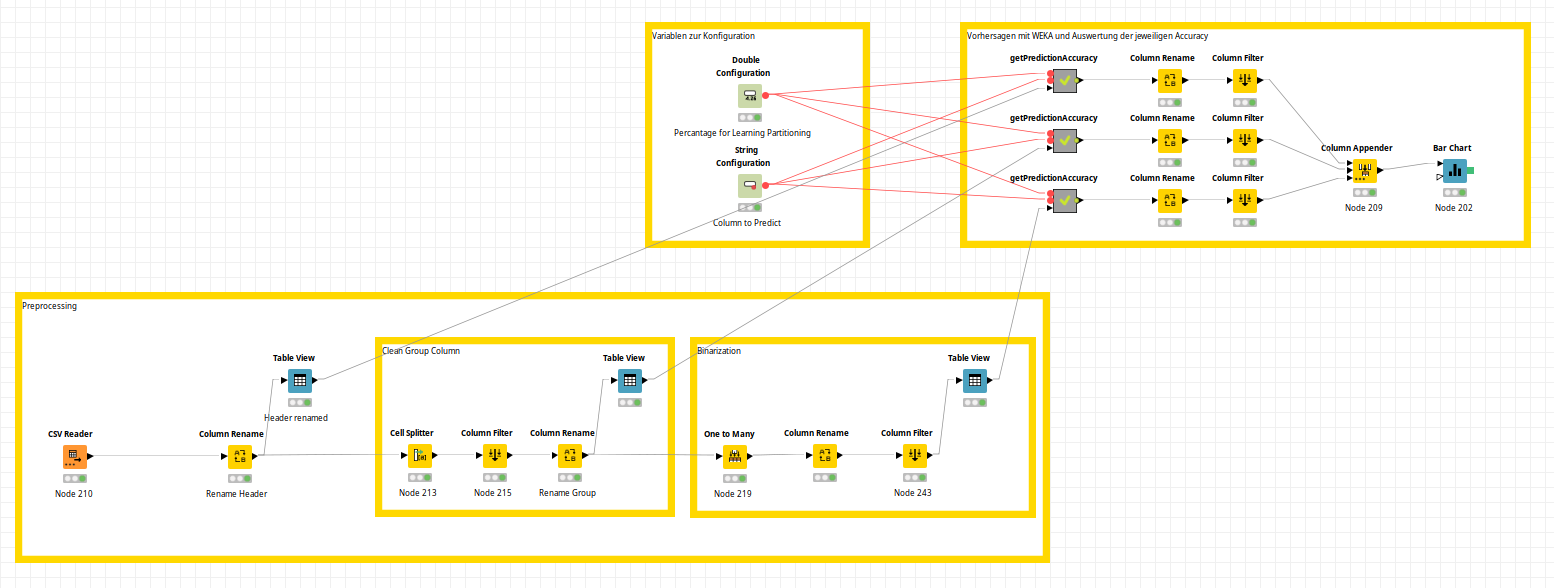
\includegraphics[scale=0.25]{../pictures/trees-workflow-gesamt.png}
						\caption{Gesamtworkflow}		
					\end{figure}	
				\end{center}	
			\end{frame}
			
			\begin{frame}{Ermittlung der Accuracys}
				\begin{itemize}
					\item Knoten zur Eingabe von:	
					\begin{itemize}
						\item vorherzusagender Spalte
						\item Trainingsdatenaufteilung
					\end{itemize}	
					\item Extrahierung der Accuracys und Anzeige in Balkendiagramm
				\end{itemize}
				\begin{center}					
					\begin{figure}[h]
						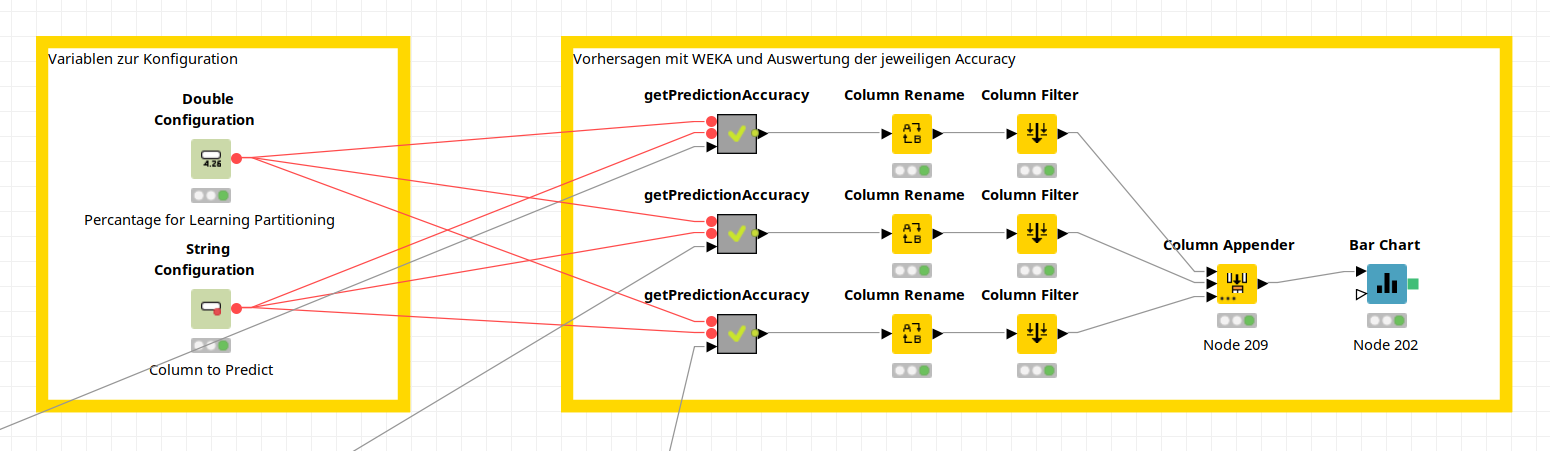
\includegraphics[scale=0.2]{../pictures/trees-workflow-gesamt-zoomed.png}
						\caption{Ermittlung der Accuracys}		
					\end{figure}	
				\end{center}	
			\end{frame}
			
			\begin{frame}{Metaknoten `getPredictionAccuracy'}
				\begin{itemize}
					\item Aufteilung in Trainings und Testdaten	
					\item Extrahierung der Accuracys
				\end{itemize}
				\begin{center}					
					\begin{figure}[h]
						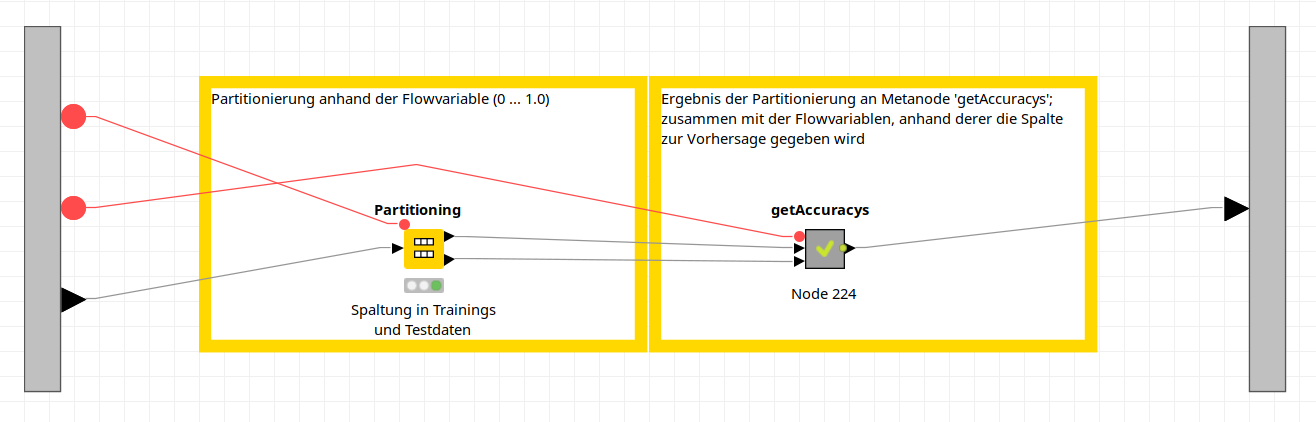
\includegraphics[scale=0.25]{../pictures/trees-workflow-partitioning.png}
						\caption{Inhalt des Metaknoten `getPredictionAccuracy'}		
					\end{figure}	
				\end{center}	
			\end{frame}
			
			\begin{frame}{Metaknoten `getAccuracys'}		
				\begin{columns}[T]
   				\begin{column}{.5\textwidth}
					\begin{itemize}
						\item Metaknoten für verschiedene Entscheidungsbäume 
						\item Gleiche Trainings- und Testmenge
						\item Zusammenführung der Accuracys in eine Tabelle
					\end{itemize}
    				\end{column}    				
    				\begin{column}{.5\textwidth}
					\begin{figure}[h]
						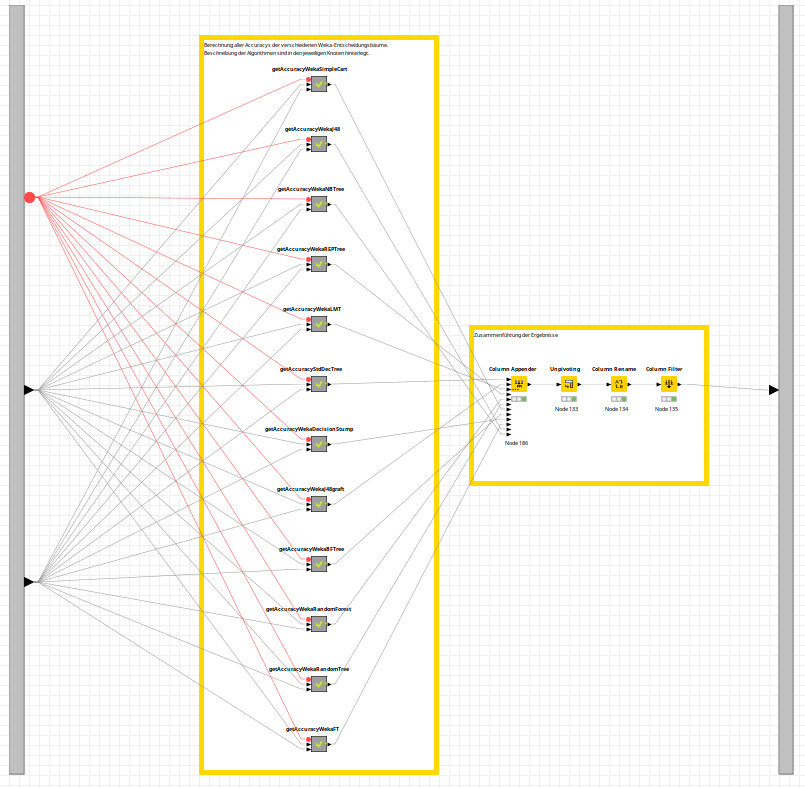
\includegraphics[scale=0.17]{../pictures/trees-workflow-getAccuracys.png}
						\caption{Inhalt des Metaknoten `getAccuracys'}			
					\end{figure}					
    				\end{column}
  				\end{columns}
			\end{frame}
			
			\begin{frame}{Beispielhafter `getAccuracyWeka*' Knoten}		
				\begin{itemize}
					\item Lerner	
					\item Vorhersage
					\item Scoring
					\item Extahierung der Accuracy
				\end{itemize}
				\begin{center}					
					\begin{figure}[h]
						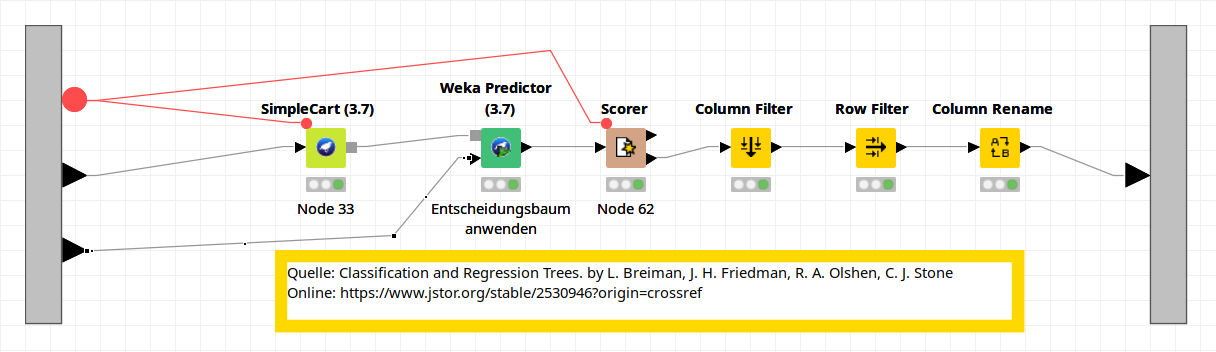
\includegraphics[scale=0.25]{../pictures/trees-workflow-weka-example.png}
						\caption{Inhalt des Metaknoten `getAccuracyWekaSimpleCart'}		
					\end{figure}	
				\end{center}	
			\end{frame}
			
			\begin{frame}{Accuracy Chart}		
				\begin{center}					
					\begin{figure}[h]
						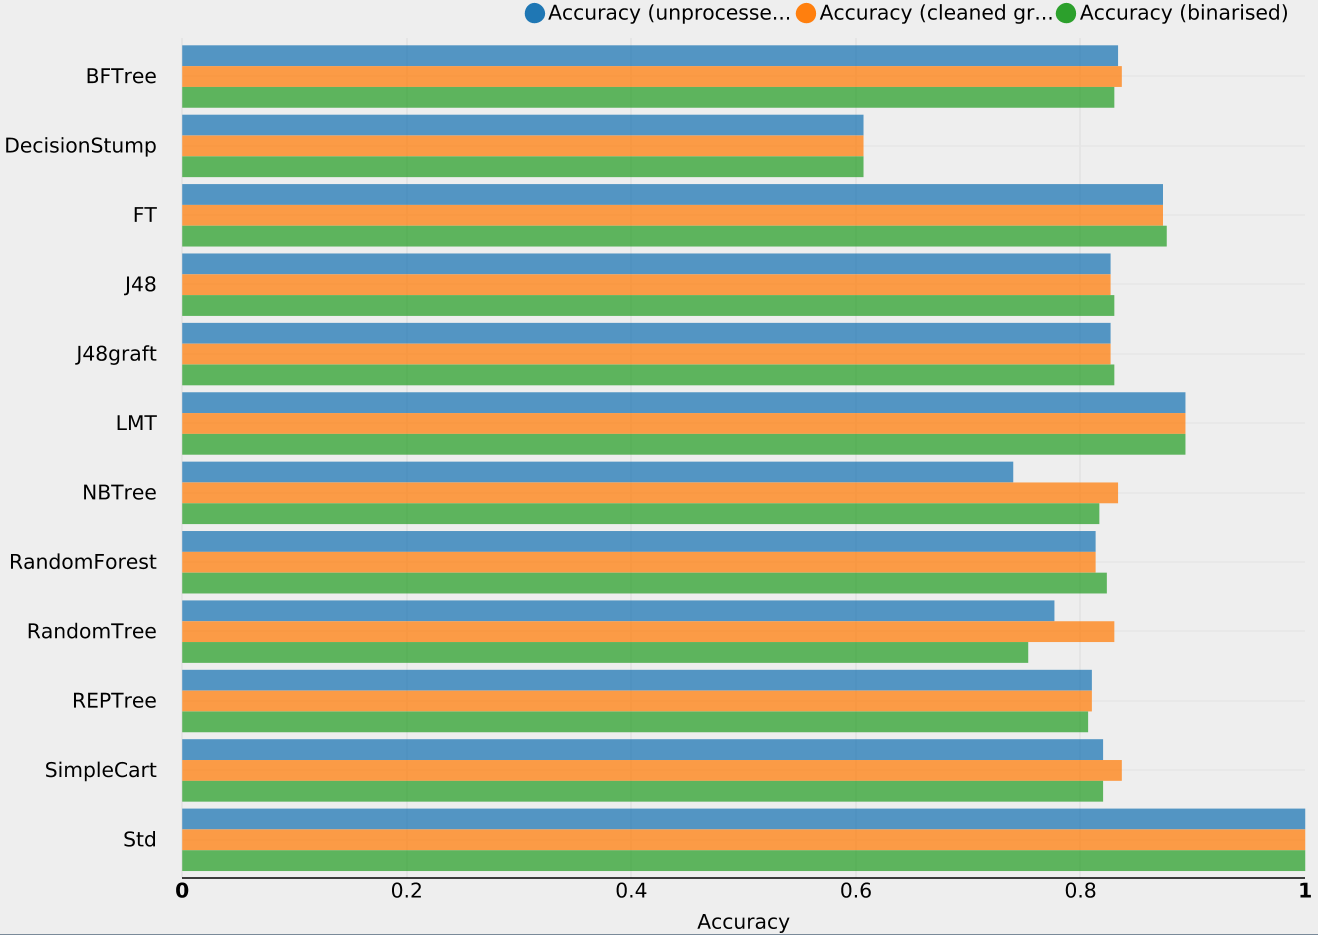
\includegraphics[scale=0.15]{../pictures/chart_accuracy.png}
						\caption{Balkendiagramm für `gender' und Trainingssatz von 70\%}		
					\end{figure}	
				\end{center}	
			\end{frame}
			
	\subsection{Cluster}
	\begin{frame}
	
	\end{frame}

			
\end{document}
